\section{Auswertung und Diskussion}
In den Abbildungen \ref{fig:bwsx}, \ref{fig:bwsy} und \ref{fig:bwsz} ist die Dosisverteilung in der Brustwirbelsäule in der Transversal-, Sagittal- und Frontalansicht zu sehen. In den Abbildungen ist zu erkennen, dass die $\SI{95}{\percent}$ Isodosenlinie das rot eingezeichnete PTV in den meisten Bereichen vollständig umschließt. Es ist lediglich in einem kleinen Teil des vorderen Bereichs des PTVs nicht gelungen eine Dosis von $\SI{95}{\percent}$ zu erreichen. Für eine bessere Beurteilung ist das Dosis-Volumen-Histogramm in der Abbildung \ref{fig:bwsdvh} gezeigt. Anhand der DVH Kurve für das PTV (rot) ist zu erkennen, dass lediglich in einem kleinen Teil des PTVs es nicht gelungen ist eine Dosis von $\SI{95}{\percent}$ zu erreichen. Die minimale Dosis, die im PTV deponiert wird, liegt bei  $\SI{86.5}{\percent}$ Isodosenlinie und es werden trotzdem  $\SI{93.58}{\percent}$ Isodosenlinie des Volumens des PTVs von der  $\SI{95}{\percent}$ Isodosenlinie umschlossen.
Im Fokus stehen hier eine Schonung der Risikoorgane als auch eine möglichst schonende Behandlung. Hierbei ist die bestmögliche PTV Erfassung nicht entscheidend wie bei einer kurativen Behandlung.

\begin{figure}[h!]
	\centering
	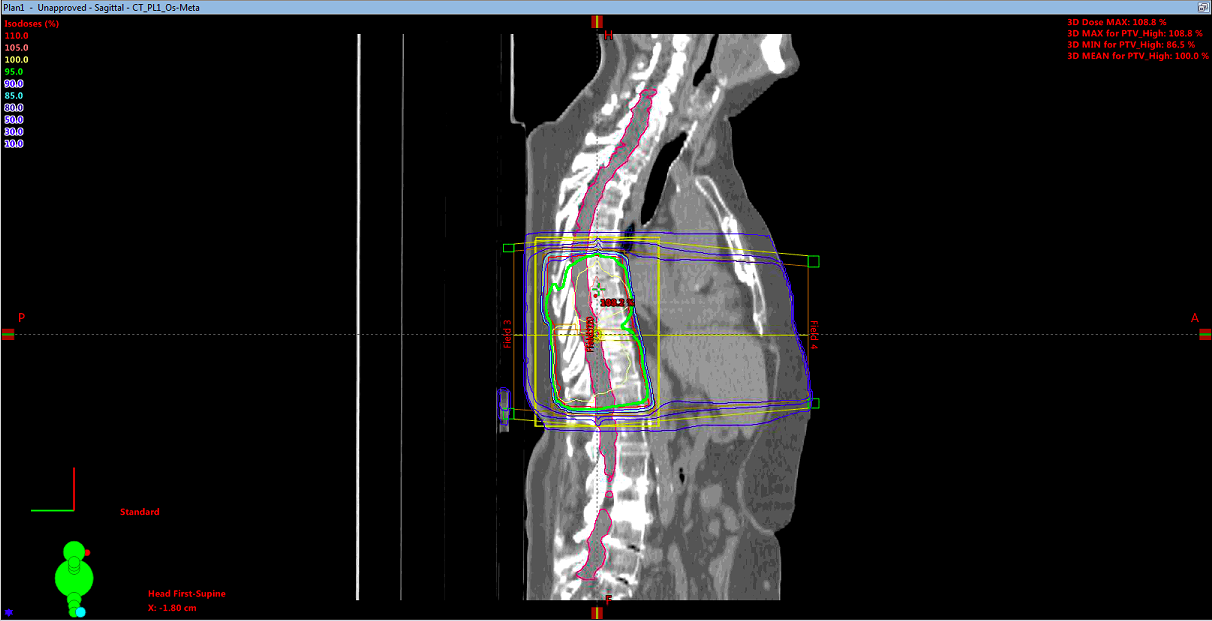
\includegraphics[width=0.7\linewidth]{Bilder/BWS_X}
	\caption{Darstellung der Dosisverteilung in der Sagittalansicht des Oberkörpers.}
	\label{fig:bwsx}
\end{figure}

\begin{figure}[h!]
	\centering
	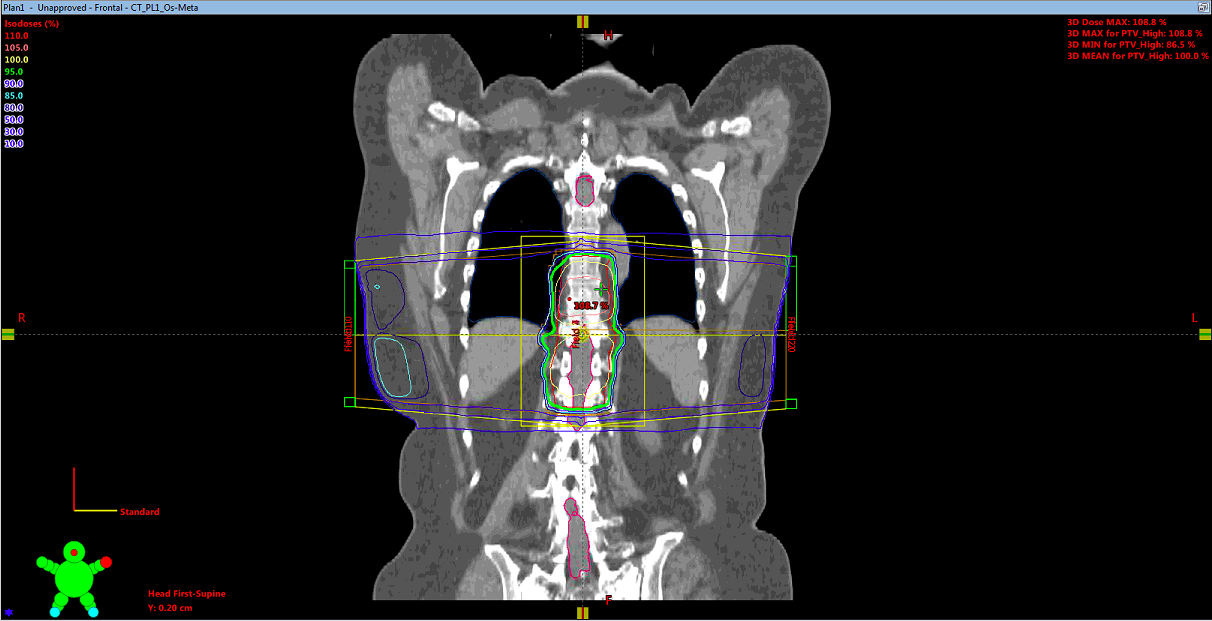
\includegraphics[width=0.7\linewidth]{Bilder/BWS_Y}
	\caption{Darstellung der Dosisverteilung in der Frontalansicht des Oberkörpers.}
	\label{fig:bwsy}
\end{figure}

\begin{figure}[h!]
	\centering
	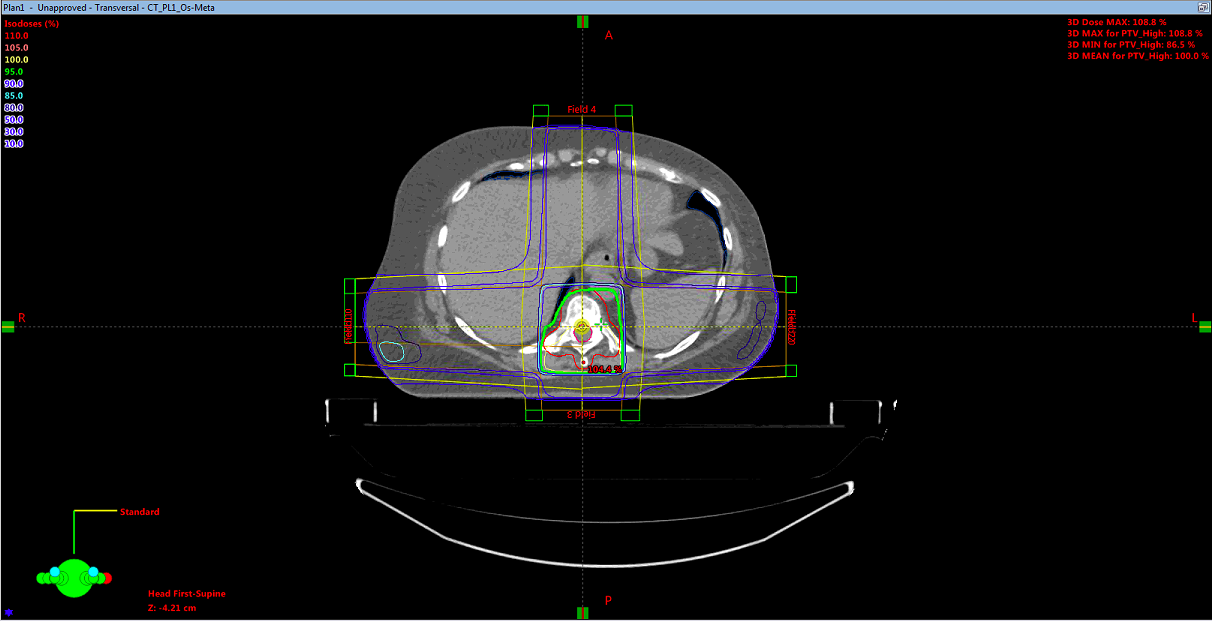
\includegraphics[width=0.7\linewidth]{Bilder/BWS_Z}
	\caption{Darstellung der Dosisverteilung in der Transversalansicht des Oberkörpers.}
	\label{fig:bwsz}
\end{figure}

Die maximale relative Dosis $\SI{108,8}{\percent}$ wird innerhalb im PTV deponiert und überschreitet die erlaubte maximale Dosis von $\SI{107}{\percent}$. Es konnte auch schon anhand der Dosisverteilung gesehen werden, dass nicht im gesamten PTV eine relative Dosis von $\SI{95}{\percent}$ erreicht werden konnte. Allerdings ist auch zu erkennen, dass nur ein sehr kleiner Teil des PTVs eine geringere Dosis als $\SI{95}{\percent}$ erhält. Anhand des DVHs des gesamten Thorax (grüne Kurve) ist zu erkennen, dass in dem gesamten Thorax nur eine relativ geringe Dosis deponiert wird. Etwa $\SI{11}{\percent}$ des Thoraxvolumens erhält eine Dosis von  $\SI{50}{\percent}$. Durch die DVH Kurven der Risikoorgane ist zu erkennen, dass sie zum Teil gut geschont werden konnten. Von den Risikoorganen erhält das Rückenmark die meiste Dosis, was bei der Lokalisation des Tumors zu erwarten war.
Die Organdosisgrenzwerte werden aus der QUANTEC Tabelle entnommen. Die mittlere Dosis der Lunge darf nicht $\SI{20}{\gray}$ überschreiten und es darf nicht mehr als $\SI{30}{\percent}$ des Lungenvolumens eine Dosis von $\SI{20}{\gray}$ erhalten. Diese Grenzwerte wurden erfolgreich eingehalten, weil nur $\SI{18,58}{\percent}$ des Volumens eine Dosis von $\SI{20}{\gray}$ erhält und die mittlere Dosis liegt bei $\SI{7,659}{\gray}$. Die rechte Lungenflügel erhält eine mittlere Dosis von $\SI{8,24}{\gray}$ und die linke Lungenflügel eine mittlere Dosis von $\SI{6,84}{\gray}$. Die mittlere Dosis der beiden Lungenflügel liegt unter dem $\SI{20}{\gray}$ Wert und auch die beiden Lungenvolumen liegen unter dem Grenzwert. Bei der rechten Lungenflügel ergibt sich bei einer Dosis von $\SI{20}{\gray}$ nur $\SI{19,37}{\percent}$, während sich bei der linken Flügel bei einer Dosis von $\SI{20}{\gray}$ nur $\SI{17,43}{\percent}$ ergibt. Der Grenzwert für die mittlere Dosis bei dem Herz beträgt $\SI{26}{\gray}$ und weniger als $\SI{46}{\percent}$ des Herzvolumens darf eine Dosis von $\SI{30}{\gray}$ erhalten. Dies wurde auch erfolgreich eingehalten, weil nur $\SI{1,22}{\percent}$ mit einer Dosis von $\SI{30}{\gray}$ bestrahlt wird und die mittlere Dosis liegt bei $\SI{14,761}{\gray}$. Bei dem Rückenmark darf die maximale Dosis $\SI{45}{\gray}$ nicht überschreiten. Bei diesem Plan liegt die maximale Dosis des Rückenmarks bei $\SI{48.94}{\gray}$ und liegt somit oberhalb des Grenzwertes. In diesem Fall ist es schwer die maximale Dosis unter dem Grenzwert einzuhalten, da das Rückenmark sich in das Zielvolumen befindet aber dennoch unter dem absoluten Grenzwert von $\SI{50}{\gray}$ liegt.
Die linke Niere beträgt eine mittlere Dosis von $\SI{6,433}{\gray}$ und die rechte eine mittlere Dosis von $\SI{4,022}{\gray}$. Hierbei darf der Grenzwert von $\SI{15}{\gray}$ bis $\SI{18}{\gray}$ für die mittlere Dosis bei den Nieren nicht überschreiten. Auch das wurde erfolgreich eingehalten. 
Die mittlere Dosis der Leber liegt bei $\SI{11,455}{\gray}$. Auch dieser Wert wurde eingehalten, da der Obergrenzwert der Leber ist bei $\SI{30}{\gray}$ bis $\SI{32}{\gray}$ laut QUANTEC. 

\begin{figure}[h!]
	\centering
	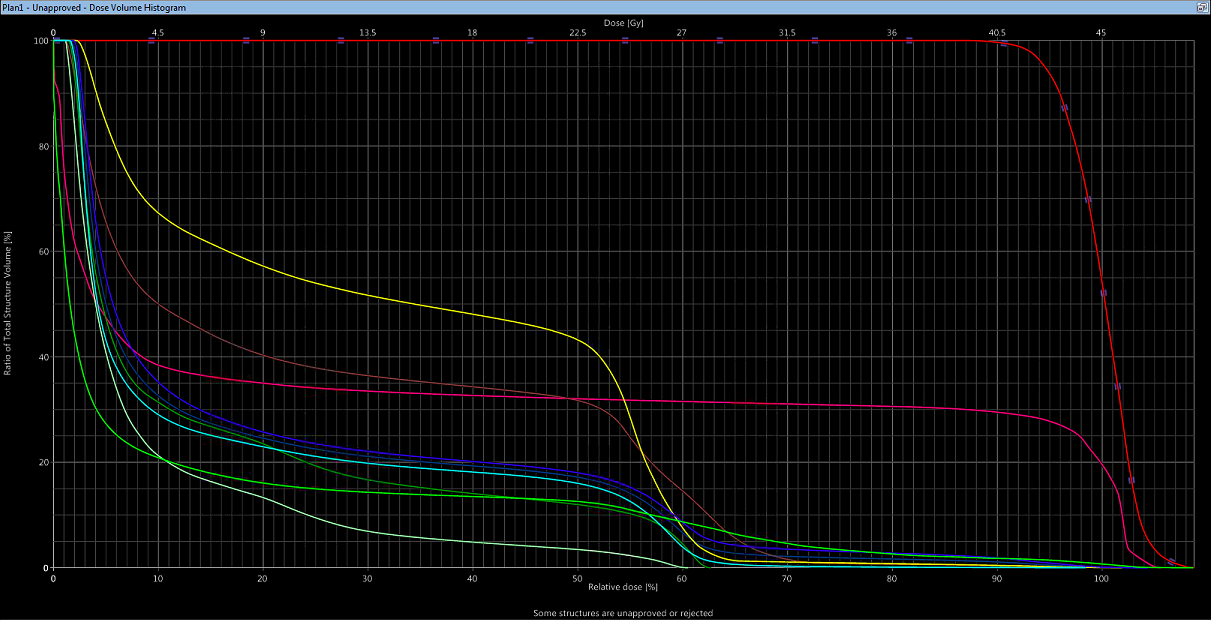
\includegraphics[width=0.7\linewidth]{Bilder/BWS_DVH}
	\caption{Zu sehen ist das Dosis-Volumen-Histogramm. In roter Farbe dargestellt ist das PTV-High und in grüner Farbe ist der gesamte Thorax. Außerdem sind noch die einzelnen Isodosenlinien eingezeichnet und die einzelnen Kurven zu den Risikoorgane wie z.B. Herz (gelb), Leber (braun), Lunge rechts (hellblau), Lunge links (blau), Lunge gesamt (dunkelblau), Niere rechts (hellgrün), Niere links(dunkelgrün) und das Rückenmark(pink).}
	\label{fig:bwsdvh}
\end{figure}

Bei dem erstellten Plan konnte nicht erreicht werden, dass das PTV komplett von der $\SI{95}{\percent}$ Isodosenlinie umschlossen wird. Das Zielvolumen, wie in den obigen Abbildungen \ref{fig:bwsx}, \ref{fig:bwsy} und \ref{fig:bwsz} zu sehen ist, ist sehr groß. Durch die verwendeten Felder mit individuell angepassten MLCs konnten zum Teil die Organdosisgrenzwerte fast aller Risikoorgane eingehalten werden. Mit diesem Plan konnte eine adäquate Behandlung gewährleistet werden. 